\documentclass{article}
\usepackage{amsmath, amssymb, amsthm}
\usepackage{graphicx}
\usepackage{listings}
\usepackage{xcolor}
\usepackage[utf8]{inputenc}
\usepackage[russian]{babel}
\usepackage{booktabs}
\usepackage{float}
\usepackage{caption}
\usepackage[T1,T2A]{fontenc}
\usepackage{minted}

\begin{document}

\section*{Расчетно графическая работа по функциональному анализу}

Выполнил студент группы М80-308Б-22 Караев Тариел Жоомартбекович.

\subsection*{Задание II}
Проведите ортогонализацию системы функций $x_n(t)=t^{n-1}$ в пространстве квадратично суммируемых функций относительно склярного произведения $\langle x, y\rangle=\int_a^b x(t) y(t) f(t) d t$. Найдите приближение функции $y$ частичной суммой ряда Фурье, обеспечивающее среднеквадратичную точность разложения $\varepsilon \in\left\{10^{-1}, 10^{-2}, 10^{-3}\right\}$ (при достаточных вычислительных ресурсах). Постройте график функции $y(t)$ и его приближения частичными суммами ряда Фурье. Продемонстрируйте несколько графиков, получающихся при промежуточных вычислениях.

\subsection*{Вариант 9}

\begin{gather*}
    k = 8, l = 5, \\
    [a, b] = \left[-0,8 - \frac{k}{10}; 0,8+\frac{k}{10}\right],
    f(t) = \frac{4l}{5} - t^2,
    y(t)= \cos(3t) \Rightarrow
\end{gather*}

\begin{gather*}
    \Rightarrow [a, b] = \left[-1,6; 1,6\right], f(t) = 4 - t^2, y(t)=\cos(3t)
\end{gather*}


\subsection*{Решение}

\begin{enumerate}
    \item Проведём ортогонализацию системы функций \( x_n(t) = t^{n-1} \) на отрезке \([-1{,}6; 1{,}6]\) с весом \( f(t) = 4 - t^2 \) с помощью метода Грамма–Шмидта.
    \item Построим ортонормированный базис.
    \item Выполним разложение функции \( y(t) = \cos(3t) \) в ряд Фурье по полученному базису.
    \item Найдём частичные суммы ряда Фурье, соответствующие точностям \( \varepsilon \in \{10^{-1}, 10^{-2}, 10^{-3} \} \).
    \item Построим графики функции и её приближений при разных значениях \( n \).
\end{enumerate}

\subsubsection*{Код программы на языке программирования Python}
\begin{minted}{python}
import numpy as np
import matplotlib.pyplot as plt
from scipy.integrate import quad
import os


a, b = -1.6, 1.6
weight = lambda t: 4 - t**2
inner = lambda f, g: quad(lambda t: f(t) * g(t) * weight(t), a, b, epsabs=1e-9)[0]

y = lambda t: np.cos(3 * t)


def poly_basis(n):
    return [lambda t, k=k: t**k for k in range(n)]


def gram_schmidt(basis):
    ortho = []
    for v in basis:
        w = v
        for u in ortho:
            proj_coeff = inner(w, u) / inner(u, u)
            w = lambda t, w=w, u=u, c=proj_coeff: w(t) - c * u(t)
        ortho.append(w)
    return ortho


def normalize(f):
    norm = np.sqrt(inner(f, f))
    return lambda t, f=f, norm=norm: f(t) / norm


def orthonormal_basis(n):
    raw = poly_basis(n)
    ortho = gram_schmidt(raw)
    return [normalize(f) for f in ortho]


def fourier_approx(y, ortho_basis):
    coeffs = [inner(y, phi) for phi in ortho_basis]
    return lambda t: sum(c * phi(t) for c, phi in zip(coeffs, ortho_basis)), coeffs


def mse(f, g):
    err = lambda t: (f(t) - g(t))**2 * weight(t)
    return np.sqrt(quad(err, a, b, epsabs=1e-9)[0])


if __name__ == '__main__':
    t_vals = np.linspace(a, b, 400)
    y_vals = y(t_vals)
    epsilons = [1e-1, 1e-2, 1e-3]
    epsilon_labels = {1e-1: "eps < 1e-1", 1e-2: "eps < 1e-2", 1e-3: "eps < 1e-3"}
    achieved_eps = {}

    os.makedirs("graphs", exist_ok=True)

    plt.figure(figsize=(12, 8))
    plt.plot(t_vals, y_vals, label='y(t) = cos(3t)', lw=2, color='black')

    intermediate_ns = [3, 5, 7, 9, 11]

    for n in intermediate_ns:
        ortho = orthonormal_basis(n)
        approx_func, _ = fourier_approx(y, ortho)
        approx_vals = [approx_func(t) for t in t_vals]
        error = mse(y, approx_func)

        for eps in epsilons:
            if eps not in achieved_eps and error < eps:
                achieved_eps[eps] = n

        plt.plot(t_vals, approx_vals, label=f"n={n}, ошибка={error:.1e}")

    print("Достижение заданных точностей:")
    for eps in epsilons:
        if eps in achieved_eps:
            print(f"Для eps = {eps:.0e}: n = {achieved_eps[eps]}")
        else:
            print(f"❌ Не достигнута точность eps = {eps:.0e}")

    plt.title("Промежуточные приближения функции y(t) частичными суммами ряда Фурье")
    plt.xlabel("t")
    plt.ylabel("y(t)")
    plt.legend()
    plt.grid(True)
    plt.tight_layout()
    plt.savefig("graphs/fourier_approximations.png")
    plt.show()
\end{minted}

\subsubsection*{Вывод программы}
Консоль:
\begin{verbatim}
Достижение заданных точностей:
Для eps = 1e-01: n = 7
Для eps = 1e-02: n = 9
Для eps = 1e-03: n = 11
\end{verbatim}

Графики:
\begin{figure}[h!]
    \centering
    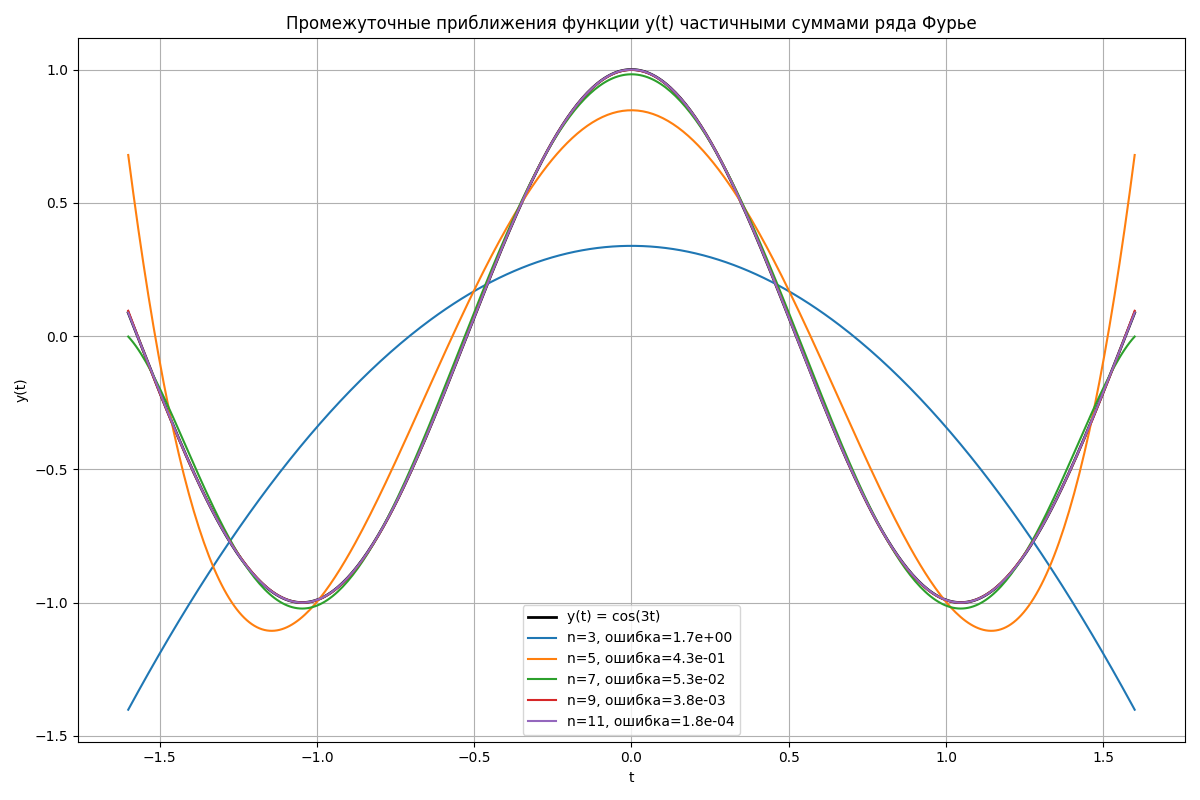
\includegraphics[width=0.7\textwidth]{fourier_approximations.png}
    \caption{Приближение функции \( y(t) = \cos(3t) \) частичными суммами ряда Фурье для различных значений \( n \)}
    \label{fig:fourier_approximations}
\end{figure}

\subsection*{Вывод}

На основе графиков (см. Рис 1) видно, что с увеличением числа членов ряда Фурье приближение функции \( y(t) = \cos(3t) \) становится всё более точным. Согласно вычислениям, для достижения точности \( \varepsilon = 10^{-1} \) достаточно 7 членов, для \( 10^{-2} \) — 9, а для \( 10^{-3} \) — 11 членов ряда. Это подтверждается как численно, так и визуально по построенным графикам.

\end{document}
